\documentclass[a4paper, 12pt, french]{article}
\usepackage[utf8]{inputenc}
\usepackage{xcolor}
\usepackage{hyperref}
\usepackage{graphicx}
\usepackage{hyphenat}
\usepackage[left=20mm, right=20mm]{geometry}
\usepackage{biblatex}
\usepackage[T1]{fontenc}
\addbibresource{Bibliographie.bib}

\title{TER (Titre ? mise en forme première page ? Logo UVSQ ? Tête et pied de page ?)}
\author{Cambresy Florian \\ Chalaud Jean-Christophe \\ Le Denmat Mickael}
\date{(date)MM YYYY}

\begin{document}
	\maketitle
	\renewcommand{\contentsname}{Table des matières}
	\newpage
	\tableofcontents

	\newpage
	\section{Développement d'une méthode e recherche arborescence pour Développement d'une méthode de recherche
	arborescence pour un jeu à deux joueurs: application au jeu 7 Wonder-Duel}
	\subsection{Sujet}
	Il s’agira tout d’abord pour les étudiants de se familiariser avec les méthodes de recherche arborescente
	appliquées aux jeux, en particulier la méthode alpha-bêta.

	Dans un second temps, il conviendra d'implémenter une telle méthode pour un jeu intitulé 7wonders - Duel.
	Ce jeu est décrit sur de nombreux sites, certains proposent même une petite vidéo tutorielle expliquant
	les règles de ce jeu. Il est à noter que l’encadrant offrira ce jeu aux étudiants qui
	choisiront ce sujet (oh, le beau cadeau).

	Pour que le programme “joue bien”, il conviendra en particulier de réfléchir à des fonctions d'évaluation
	pertinentes des positions de jeu.

	\subsection{Description du travail attendu}
	L'objectif du projet est d'implémenter une méthode alpha-bêta pour faire en sorte que notre algorithme puisse
	jouer, en proposant des coups "intelligents", dignes d'intérêts. Nous expliquerons bien evidement qu'est ce que
	nous considérons comme étant un coup digne d'intérêts et sur quels critères ce base notre algorithme.

	Afin d'apporter une solution à ce sujet, nous découperons le projet en trois parties.

	La première sera une partie descriptive concernant les notions contenues dans la méthode alpha-bêta pour
	le programme joue correctement en insistant sur les points qui devront être étudiés afin d'appliquer la méthode
	à notre exemple précis. Ensuite, nous expliquerons les règles du jeu et évoquerons le déroulement d'une partie.
	Nous développerons sur le système de victoire et, afin de faire une transition sur la partie qui suivra, nous
	débattrons concernant la force des "positions" au cours d'une partie.

	La deuxième partie montrera le chemin de pensée que nous avons eu afin d'arriver à une ou des solutions pour
	appliquer la méthode alpha-beta sur notre jeu. Plus particulièrement nous décrirons la fonction d'évaluation
	que nous avons trouvé afin que l'algorithme suggère des coups "intelligents".

	Enfin la dernière sera une présentation des solutions techniques que nous avons du mettre en place.

	\subsection{Description du jeu : 7 wonders-Duel}
	7 Wonder est un jeu de plateau sorti dans les années 2010 créé Antoine Bauza et publier par Repos Production en
	Belgique. Le nombre de joueur est entre 3 et 7. Un jeu où l'on joue une ancienne
	civilisation avec ces conflits milaitaires mais aussi ces activites de commerce. Il est connu et très apprécié
	par la communauté ayant remporté plus de 30 prix et souvent cité comme l'un des jeux de société les plus influents
	de la dernière décennie\cite{wiki_7_wonder}.
	Le choisit afin d'appliquer l'algorithme min-max est une variante de ce jeu, le 7 wonders - Duel.

	\subsubsection{7 wonders - Duel}
	Le jeu 7 wonders - Duel est comme son nom l'indique un 7 wonders mais à deux joueur. Un jeu sortie en 2015
	par la même société. \textcolor{red}{A DVP ?}

	\subsubsection{Règles du jeu}
	Le jeu se présente comme suit dans le livret des règles\cite{regle_7_wonder_duel}.
	\textcolor{red}{PRENDRE EN PHOTO LE JEU AU DEBUT DE LA PARTIE}.

	Il est constitué de:
	\begin{itemize}
		\item 1 plateau de jeu. \textcolor{red}{IMAGE ?}
		\item 66 cartes Âge. \textcolor{red}{IMAGE ?}
		\begin{itemize}
			\item 23 cartes pour l'Âge I.
			\item 23 cartes pour l'Âge II.
			\item 20 cartes pour l'Âge III.
		\end{itemize}
		\item 7 cartes Guilde.
		\item 12 cartes Merveille, avec un nom, un coût en ressource et un effet (un bonus). \textcolor{red}{IMAGE ?}
		\item 4 jetons Militaire, donnant une certaine somme de monnaie. \textcolor{red}{IMAGE ?}
		\item 10 jetons Progrès. \textcolor{red}{IMAGE ?}
		\item 1 Pion Conflit, indiquant quel joueur a l'avantage militaire. \textcolor{red}{IMAGE ?}
		\item 31 pièces de monnaie \textcolor{red}{IMAGE ?}
		\begin{itemize}
			\item 14 de valeur 1.
			\item 10 de valeur 3.
			\item 7 de valeur 6.
		\end{itemize}
		\item 1 carnet de scores.
	\end{itemize}

	Les cartes Âge et Guilde sont des bâtiments. Elles peuvent avoir un coût (monnetaire) afin d'être
	utilisée, qui placé en haut à gauche. Elles peuvent donner des effets, placé en haut au centre.
	Les effets sont multiple comme par exemple une production de matière, une réduction de coût de construction
	d'un bâtiment ou d'une merveille, ainsi que d'autres. Enfin elles ont aussi un nom, placé en bas. Les cartes
	ont des couleurs différentes indiquant à quel type de bâtiment elles appartiennent.
	\begin{itemize}
		\item Les Cartes marrons sont des bâtiments de matière première.
		\item Les Cartes grises sont des bâtiments de produit manufacturé.
		\item Les cartes bleues sont des bâtiments civils, ils donnent des points de victoire.
		\item Les cartes vertes sont des bâtiments scientifiques, ils donnent aussi des points de victoire et
		\item un symbole scientifique. Lorsqu'un joueur a deux symbole scientifique identique
		\item il peut prendre un jeton Progres.
		\item Les cartes oranges sont des bâtiments commerciaux, ils ont des objectifs multiples comme donner
		\item des pièces au joueur, produire des ressources, modifier les règles de commerce.
		\item Les cartes rouges sont des bâtiments militaires, ils augmentent la puissance.
		\item Les cartes violettes sont des bâtiment de Guilde, ils donnent des points de victoire en fonction
		\item de certains critères.
	\end{itemize}

	De plus le joueur peut acheter des ressources à la "banque" via le commerce. Par exemple si le joueur souhaite
	construire un bâtiment mais il ne dispose pas de toutes les ressouces. Pour acheter cette ressource il faut prendre
	en compte les ressources produite par le joueur advairse (carte marron et grise) et ajouter 2 et remettre la somme
	à la banque puis construire le bâtiment. Concernant les bâtiments, certains octroient un symbole de chaînage
	(en blanc en haut de la carte). Si le joueur prend souhaite construire un bâtiment et si il possède une carte
	donnant le symbole de chaînage il peut alors construire gratuitement le bâtiment, dans le cas contraire
	il devrait payer son coût en ressources et/ou monnetaire.

	Une fois la présentation fait, nous allons pouvoir parler de la préparation du jeu avant de débuter une partie.
	La préparation du plateau de se fait ainsi:
	\begin{enumerate}
		\item Placez le plateau entre les deux joueurs.
		\item Placez le pion Conflit sur la case neutre au milieu du plateau.
		\item Placez les quatres jetons Militaire sur leurs emplacements.
		\item Mélangez les jetons Progrès et placez-en cinqs au hasard sur la plateau.
		\item Chaque joueur prend 7 pièce à la banque.
	\end{enumerate}

	Puis vient la selection des Merveilles, pour cela il faut désinger le premier joueur et mélanger les Merveilles,
	ensuite:
	\begin{itemize}
		\item Disposez 4 Merveilles aléatoires entre les joueurs.
		\item Le premier joueur choisit une Merveille.
		\item Le deuxième joueur en choisit deux.
		\item Le premier joueur prend la dernière.
		\item Disposez les quatres autres Merveilles.
		\item Le deuxième joueur choisit une Merveille.
		\item Le premier joueur en choisit deux.
		\item Le deuxime joueur prend la dernière.
	\end{itemize}
	Pour construire une Merveille, le joueur doit mettre une carte face caché sous la Merveille (peut importe
	la carte, elle sert juste a indiquer qque la Mereveille est construite) et doit payé le coup de la construction.
	Il y a un maximum de 7 Merveille construite par partie, le joueur dont la dernière Merveille n'est pas construite
	doit la remettre dans la boite.

	Enfin il faut placer les cartes d'Âge dans une structure particulière en fonction de l'âge. Les cartes facent
	cachées sont retournées lorsque les cartes visibles posées dessus sont enlevées par les joueurs. Les joueurs
	peuvent choisir aussi de défausser une carte en échange de 2 pièces et d'un bonus d'une pièce pour chaque carte
	jaune qu'il possède.

	Il y a deux manières de gagner, la première est la victoire militaire, l'un des joueur aura avancé le pion
	Conflit dans la case capitale de son adversaire. La deuxième étant la victoire par suprémactie scientifique,
	l'un des joueur réunit 6 symboles scientifiques différents. Si aucun des joueur n'a gagner à la fin de l'Âge III,
	il faut alors faire la sommes des points de victoire acquis durant la partie, celui qui en possde le plus l'emporte.

	\section{Rappels généraux}
	\subsection{Théorie des jeux}
	Dans le monde des mathématiques il existe un domaine qui s'intéresse aux interactions stratégiques qui existent
	entre plusieurs agents. Ces interactions peuvent se faire dans un jeu, dans les sciences sociales, politiques
	ainsi que dans d'autres exemples. Ce domaine est la théorie des jeux\cite{wiki_theorie_jeux}.
	Il faut noter que ici le mot "jeu" a un sens plus large qu'un jeu de société ou autre.

	Dans ce projet nous porterons attention uniquement aux interactions entre deux joueurs dans un jeu de société à
	travers un exemple que nous développerons par la suite.

	\subsection{Catégories de jeux}
	Afin de connaître quelle approche doit être utilisée pour étudier les stratégies qui existent au sein d'un jeu,
	la théorie repartie les jeux en différentes catégories\cite{wiki_typo_theorie_jeux}.
	\begin{enumerate}
		\item Coopératifs ou non.
		\item Somme nulle ou non.
		\item Simultanés ou séquentiels.
		\item Information complète ou non.
		\item Mémoire parfaite ou non.
		\item Determiné.
		\item Finis.
		\item Répétés.
	\end{enumerate}
	(1) Un jeu coopératif permet d'analyser la formation de coalitions afin d'améliorer le gain potentiel. \\
	(2) Un jeu à somme nulle (ou jeu strictement compétitif) est un jeu dont les gains de certains joueurs
	sont les pertes des autres afin d'avoir la somme des gains et des pertes nulles, comme dans les échecs,
	dans le poker ou dans d'autres. A l'inverse dans un jeu à somme non nulle, tous les joueurs peuvent perdre,
	ou gagner, voir même certains peuvent gagner un gain moins (réciproquement plus) important que la perte totale
	d'autres joueurs.\\
	(3) Un jeu est dit "simultané" si les joueurs jouent en même temps, dans le cas contraire c'est un jeu séquentiel.\\
	(4) Un jeu peut être à "information complète", c'est-à-dire que chaque joueur connait l'ensemble des informations
	qui influent leur prise de décision.\\
	(5) Un jeu peut être aussi à "mémoire parfaite", dans ce cas chaque joueur peut se rappeler des coups qui ont été
	joués soit en les notant a part, soit ils sont visibles au cours de la partie (par exemple les cartes qu'a choisie
	le joueur sont à coté de ce dernier, face visible).\\
	(6) Un jeu "déterminé" est un jeu particulier à somme nulle sans intervention du hasard.

	\subsection{Représentation d'un jeu}
	Maintenant que nous savons comment définir un jeu, nous allons étudier comment représenter ce dernier et les
	interactions entre les joueurs. Il existe globalement trois représentations\cite{wiki_representation_theorie_jeux}
	, la forme extensive et la forme normale, qui sont utilisées pour les jeux non coopératifs et
	la forme caractéristique pour les jeux coopératifs.

	\subsubsection{forme extensive}
	La forme extensive est la représentation sous forme d'arbre de décision où les noeuds d'une même hauteur sont les
	choix possibles (qui ne sont pas en dehors des règles prévues par le jeu) d'un joueur. Plus précisément chaque
	noeud est une situation produite au cours d'une partie (pas nécessairement le début de la partie) et les fils de
	ce noeud sont les coups que peut faire le joueur suivant. Par exemple dans les échecs, la racine sera l'état du
	plateau de jeu à la fin du tour d'un joueur (la position des pions de chaque joueur) et les fils de cette racine
	seront les déplacements des pions de l'adversaire. Dans cet exemple, ainsi que dans tous les joueurs à deux joueurs,
	les hauteurs paires sont les coups du joueur A tandis que les hauteurs impaires sont les coups du joueur B.
	De plus, les feuilles de cet arbre sont des noeuds indiquant la fin de la partie, soit il y a victoire d'un des
	deux joueurs, soit plus aucun coup n'est possible.
	C'est la forme que nous allons utiliser durant tout ce projet, c'est pour cela que nous passerons rapidement sur
	les autres formes.

	\subsubsection{forme normale}
	La forme normale (ou stratégique) est définie par:
	\begin{itemize}
		\item L'ensemble des joueurs (de taille fini).
		\item L'ensemble des stratégies possibles pour chacun des joueurs (fini ou infini).
		\item Les préférences de chacun des joueurs, soit un sous-ensemble de stratégies parmi l'ensemble des
		\item combinaisons stratégiques possibles soit via une fonction d'utilité ou un fonction de gain.
	\end{itemize}
	\textcolor{red}{A CREUSER ?}

	\subsubsection{forme caractéristique}
	La forme caractéristique est utilisée, comme dit précédememnt, pour les jeux coopératifs. Elle est représentée
	sous forme d'un graphe G=(N,v) avec N l'ensemble des joueurs et v la fonction caractéristique. Cette dernière
	associe à chaque sous-ensemble de joueurs (noté S) qui forme une coalition, la valeur v(S), la gain obtenu
	par la coalition. \textcolor{red}{A CREUSER ?}

	\subsection{Recherche arborescente et intelligence artificielle}
	La recherche arborescente est une recherche qui se base sur la forme extensive afin d'utiliser l'arbre de
	décision\cite{cours_arbre_decision}.
	Cette recherche s'appuie aussi sur une fonction d'évaluation, qui associe à toutes situations du jeu une
	valeur indiquant si elle est favorable à une victoire. Bien évidemment plus cette valeur est grande plus
	la probabilité de victoire est grande. Cette fonction ne s'applique qu'aux feuilles de l'arbre de décision,
	ces feuille peuvent être la fin de la partie ou un état de la partie dans lequel nous évaluons le rapport de force
	entre les deux joueurs afin de déterminer qui est en meilleur posture pour gagner. Ainsi l'objectif de cette
	recherche est de choisir la suite de noeud à prendre (donc de coups à faire) afin d'arriver à la valeur
	d'évaluation maximale.

	\subsection{Méthode alpha-bêta}
	\subsubsection{Méthode min-max}
	Avant d'évoquer la méthode alpha-bêta, nous allons expliquer comment fonctionne la méthode min-max,
	la méthode alpha-bêta en est une amélioration. La méthode min-max est un algorithme utilisé dans la théorie des
	jeux, plus précisément dans les jeux à deux joueurs, à somme nulle et à information complète\cite{min_max}.

	L'objectif de cette dernière est de minimiser la perte dans le pire cas pour un joueur est de maximiser
	la perte pour l'adversaire, d'où son nom "min-max". Pour cela l'algorithme va simuler tous les coups
	possibles et leur donner une valeur, représentant combien ce coup est intéressant ou non.
	La simulation de tous les coups possibles passe par la construction de l'arbre de décision et
	le calcul de la valeur des feuilles est l'application d'une fonction d'évaluation. Nous obtenons donc
	un arbre avec des valeurs aux feuilles uniquement. Ensuite, nous allons devoir faire "remonter" la valeur
	du jeu des feuilles jusqu'à la racine et choisir parmi tous les coups celle qui a la valeur la moins basse. Pour
	calculer cette valeur nous allons passer par une approche récursive comme suit\cite{minimax_alog}:
	\begin{itemize}
		\item minmax(p) = f(p) si p est un feuille de l'arbre où f est la fonction d'évaluation.
		\item minmax(p) = max(minmax(O$_1$), \ldots, minmax(O$_n$)) si p est un noeud de l'ordinateur avec les
			fils O$_1$, \ldots, O$_n$.
		\item minmax(p) = min(minmax(O$_1$), \ldots, minmax(O$_n$)) si p est un noeud du joueur avec les fils
			O$_1$, \ldots, O$_n$.
	\end{itemize}

	Le soucis de cette méthode est le nombre de cas à étudier. En effet comme la simulation
	produit un arbre que nous devons parcourir en entier afin de choisir le meilleur coup à jouer
	nous devons faire un parcours de cet arbre. Cependant comme cela passe soit par un algorithme récursif,
	qui doit simuler un nombre important de coups et de réponses ce qui fait augmenter la profondeur de l'arbre.
	En plus de faire augementer le nombre d'appel récursif cela surcharge le tas d'appel. Soit, dans l'autre cas,
	nous pouvons passer par un algorithme itératif avec une file ou une pile. Or si le nombre de réponses possibles
	à un coup du joueur devient trop important cela nous oblige à utiliser beaucoup de mémoire. Enfin, même si nous
	prévoyons le fait que le programme utilise beaucoup de mémoire, nous ne voulons pas que le programme continue de
	calculer une suite de coups qui est moins avantageuse une suite qu'il à déjà calculé. Cela serai contre-productif.
	Ainsi c'est pour répondre à toutes ces problématiques que l'élagage alpha-bêta a été conçu.

	\subsubsection{Amélioration alpha-bêta}
	L'élagage alpha-bêta est comme son nom l'indique une méthode qui vise à "supprimer" les branches de l'arbre qui
	ne sont pas utile, qui ne change rien au résultat final. Pour élager les branches, nous disposons de deux types de
	coupures, la coupure alpha et la coupure bêta, d'où le nom de la méthode\cite{elagage_alpha_beta}
	Cette méthode s'applique uniquement sur des arbres au moins de profondeur trois
	(la racine ayant un profondeur de un). Une fois que la méthode min-max à construit l'arbre
	et appliqué la fonction d'évaluation aux feuilles, nous allons ajouter les coupures lors de la
	"remonter" des valeurs à la racine.

	\subsubsection{Coupure Alpha}
	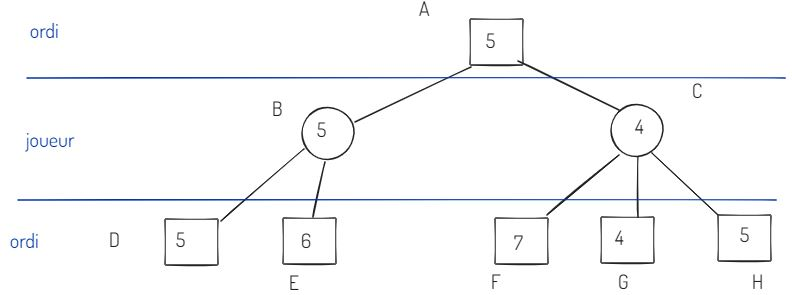
\includegraphics[width=12cm]{images/elagageAlpha.JPG}
	\textcolor{red}{A FAIRE PROPRE}

	Prenons l'exemple ci-dessus pour expliquer la coupure alpha, elle se place du point de vue du joueur.
	Une fois que la valeur du noeud B à été initialisé avec le minimum de ces fils (D, F) cette valeur va nous
	servir de borne pour faire nos coupures. Regardons les fils du frère de B, c'est à dire F, G (supposons que
	la valeur de H ne soit encore connue) afin d'initialiser la valeur de C. Nous devons prendre la valeur minimale
	entre F et G (ici F=4) mais nous constatons que cette valeur est plus petite que notre borne (B=5), ainsi explorer
	le noeud H ne sert a rien car peut importe la valeur qu'il aura (plus petite ou plus grande que F) il ne sera pas
	utiliser pour initialiser la valeur de A pusique A=max(B,C). Nous pouvons donc élaguer H (et tous les autres fils
	de C s'ils existent) comme sur l'image ci-dessous.

	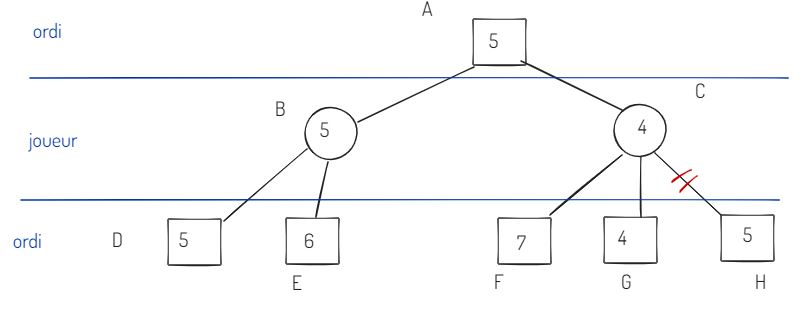
\includegraphics[width=12cm]{images/elagageAlphaSuite.JPG}
	\textcolor{red}{A FAIRE PROPRE}

	\subsubsection{Coupure Bêta}
	La coupure bêta est similaire mais se base du point de vue de l'ordinateur, on élague donc les
	feuilles plus grande que la borne\cite{wiki_7_wonder}.

	\section{Travail effectué}
	\subsection{La fonction d'évaluation}
	\subsection{Implémentation}
	\subsection{Interface}
	\subsection{Résultat obtenue}

	\section{Conclusion}
	\subsection{Objectif(s) atteint/ non atteint}
	\subsection{Suggestion d'amélioration(s)}
	\subsection{Difficultée(s) rencontrée(s)}

	\section{Annexe}
	\subsection{Code}

	\printbibliography

\end{document}
